% Options for packages loaded elsewhere
\PassOptionsToPackage{unicode}{hyperref}
\PassOptionsToPackage{hyphens}{url}
%
\documentclass[
]{article}
\usepackage{lmodern}
\usepackage{amssymb,amsmath}
\usepackage{ifxetex,ifluatex}
\ifnum 0\ifxetex 1\fi\ifluatex 1\fi=0 % if pdftex
  \usepackage[T1]{fontenc}
  \usepackage[utf8]{inputenc}
  \usepackage{textcomp} % provide euro and other symbols
\else % if luatex or xetex
  \usepackage{unicode-math}
  \defaultfontfeatures{Scale=MatchLowercase}
  \defaultfontfeatures[\rmfamily]{Ligatures=TeX,Scale=1}
\fi
% Use upquote if available, for straight quotes in verbatim environments
\IfFileExists{upquote.sty}{\usepackage{upquote}}{}
\IfFileExists{microtype.sty}{% use microtype if available
  \usepackage[]{microtype}
  \UseMicrotypeSet[protrusion]{basicmath} % disable protrusion for tt fonts
}{}
\makeatletter
\@ifundefined{KOMAClassName}{% if non-KOMA class
  \IfFileExists{parskip.sty}{%
    \usepackage{parskip}
  }{% else
    \setlength{\parindent}{0pt}
    \setlength{\parskip}{6pt plus 2pt minus 1pt}}
}{% if KOMA class
  \KOMAoptions{parskip=half}}
\makeatother
\usepackage{xcolor}
\IfFileExists{xurl.sty}{\usepackage{xurl}}{} % add URL line breaks if available
\IfFileExists{bookmark.sty}{\usepackage{bookmark}}{\usepackage{hyperref}}
\hypersetup{
  pdftitle={Class06},
  hidelinks,
  pdfcreator={LaTeX via pandoc}}
\urlstyle{same} % disable monospaced font for URLs
\usepackage[margin=1in]{geometry}
\usepackage{color}
\usepackage{fancyvrb}
\newcommand{\VerbBar}{|}
\newcommand{\VERB}{\Verb[commandchars=\\\{\}]}
\DefineVerbatimEnvironment{Highlighting}{Verbatim}{commandchars=\\\{\}}
% Add ',fontsize=\small' for more characters per line
\usepackage{framed}
\definecolor{shadecolor}{RGB}{248,248,248}
\newenvironment{Shaded}{\begin{snugshade}}{\end{snugshade}}
\newcommand{\AlertTok}[1]{\textcolor[rgb]{0.94,0.16,0.16}{#1}}
\newcommand{\AnnotationTok}[1]{\textcolor[rgb]{0.56,0.35,0.01}{\textbf{\textit{#1}}}}
\newcommand{\AttributeTok}[1]{\textcolor[rgb]{0.77,0.63,0.00}{#1}}
\newcommand{\BaseNTok}[1]{\textcolor[rgb]{0.00,0.00,0.81}{#1}}
\newcommand{\BuiltInTok}[1]{#1}
\newcommand{\CharTok}[1]{\textcolor[rgb]{0.31,0.60,0.02}{#1}}
\newcommand{\CommentTok}[1]{\textcolor[rgb]{0.56,0.35,0.01}{\textit{#1}}}
\newcommand{\CommentVarTok}[1]{\textcolor[rgb]{0.56,0.35,0.01}{\textbf{\textit{#1}}}}
\newcommand{\ConstantTok}[1]{\textcolor[rgb]{0.00,0.00,0.00}{#1}}
\newcommand{\ControlFlowTok}[1]{\textcolor[rgb]{0.13,0.29,0.53}{\textbf{#1}}}
\newcommand{\DataTypeTok}[1]{\textcolor[rgb]{0.13,0.29,0.53}{#1}}
\newcommand{\DecValTok}[1]{\textcolor[rgb]{0.00,0.00,0.81}{#1}}
\newcommand{\DocumentationTok}[1]{\textcolor[rgb]{0.56,0.35,0.01}{\textbf{\textit{#1}}}}
\newcommand{\ErrorTok}[1]{\textcolor[rgb]{0.64,0.00,0.00}{\textbf{#1}}}
\newcommand{\ExtensionTok}[1]{#1}
\newcommand{\FloatTok}[1]{\textcolor[rgb]{0.00,0.00,0.81}{#1}}
\newcommand{\FunctionTok}[1]{\textcolor[rgb]{0.00,0.00,0.00}{#1}}
\newcommand{\ImportTok}[1]{#1}
\newcommand{\InformationTok}[1]{\textcolor[rgb]{0.56,0.35,0.01}{\textbf{\textit{#1}}}}
\newcommand{\KeywordTok}[1]{\textcolor[rgb]{0.13,0.29,0.53}{\textbf{#1}}}
\newcommand{\NormalTok}[1]{#1}
\newcommand{\OperatorTok}[1]{\textcolor[rgb]{0.81,0.36,0.00}{\textbf{#1}}}
\newcommand{\OtherTok}[1]{\textcolor[rgb]{0.56,0.35,0.01}{#1}}
\newcommand{\PreprocessorTok}[1]{\textcolor[rgb]{0.56,0.35,0.01}{\textit{#1}}}
\newcommand{\RegionMarkerTok}[1]{#1}
\newcommand{\SpecialCharTok}[1]{\textcolor[rgb]{0.00,0.00,0.00}{#1}}
\newcommand{\SpecialStringTok}[1]{\textcolor[rgb]{0.31,0.60,0.02}{#1}}
\newcommand{\StringTok}[1]{\textcolor[rgb]{0.31,0.60,0.02}{#1}}
\newcommand{\VariableTok}[1]{\textcolor[rgb]{0.00,0.00,0.00}{#1}}
\newcommand{\VerbatimStringTok}[1]{\textcolor[rgb]{0.31,0.60,0.02}{#1}}
\newcommand{\WarningTok}[1]{\textcolor[rgb]{0.56,0.35,0.01}{\textbf{\textit{#1}}}}
\usepackage{graphicx,grffile}
\makeatletter
\def\maxwidth{\ifdim\Gin@nat@width>\linewidth\linewidth\else\Gin@nat@width\fi}
\def\maxheight{\ifdim\Gin@nat@height>\textheight\textheight\else\Gin@nat@height\fi}
\makeatother
% Scale images if necessary, so that they will not overflow the page
% margins by default, and it is still possible to overwrite the defaults
% using explicit options in \includegraphics[width, height, ...]{}
\setkeys{Gin}{width=\maxwidth,height=\maxheight,keepaspectratio}
% Set default figure placement to htbp
\makeatletter
\def\fps@figure{htbp}
\makeatother
\setlength{\emergencystretch}{3em} % prevent overfull lines
\providecommand{\tightlist}{%
  \setlength{\itemsep}{0pt}\setlength{\parskip}{0pt}}
\setcounter{secnumdepth}{-\maxdimen} % remove section numbering

\title{Class06}
\author{}
\date{\vspace{-2.5em}}

\begin{document}
\maketitle

\hypertarget{r-markdown}{%
\subsection{R Markdown}\label{r-markdown}}

\hypertarget{this-is-a-level-2-heading}{%
\subsection{This is a level 2 heading}\label{this-is-a-level-2-heading}}

This is regular old text!

\textbf{This creates bolded font}

and a list of stuff

\begin{itemize}
\tightlist
\item
  apples
\item
  oranges
\item
  bananas
\end{itemize}

\begin{Shaded}
\begin{Highlighting}[]
\KeywordTok{plot}\NormalTok{(}\DecValTok{1}\OperatorTok{:}\DecValTok{5}\NormalTok{, }\DataTypeTok{col=}\StringTok{"blue"}\NormalTok{, }\DataTypeTok{typ=}\StringTok{"o"}\NormalTok{)}
\end{Highlighting}
\end{Shaded}

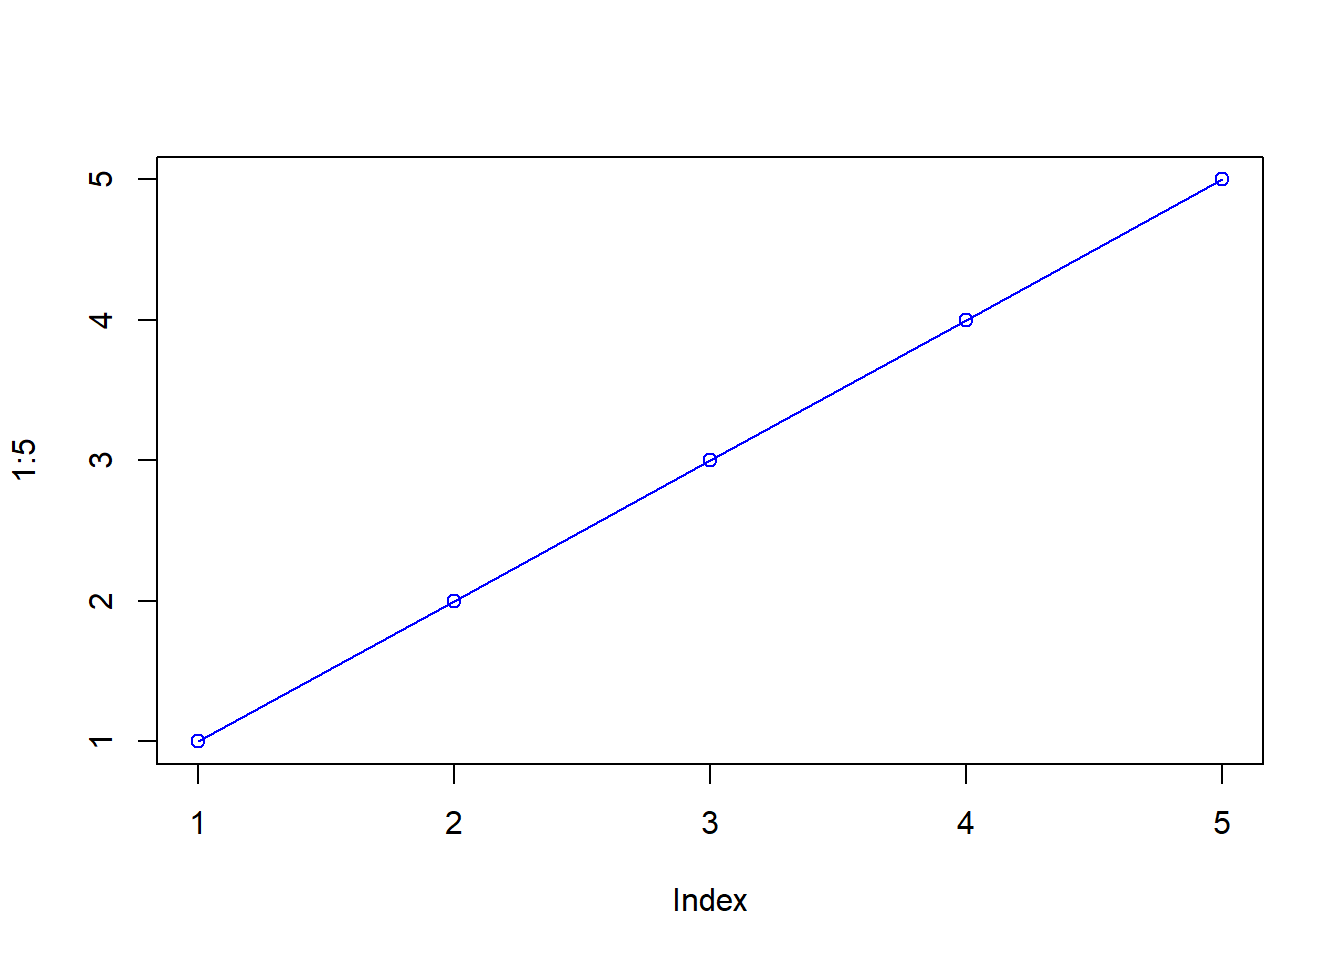
\includegraphics{Class06_files/figure-latex/unnamed-chunk-1-1.pdf}

\begin{Shaded}
\begin{Highlighting}[]
\NormalTok{x <-}\StringTok{ }\KeywordTok{c}\NormalTok{(}\DecValTok{1}\OperatorTok{:}\DecValTok{10}\NormalTok{)}
\NormalTok{x}
\end{Highlighting}
\end{Shaded}

\begin{verbatim}
##  [1]  1  2  3  4  5  6  7  8  9 10
\end{verbatim}

lets insert a code chunk with the shortcut \texttt{ctrl-alt-i}

\begin{Shaded}
\begin{Highlighting}[]
\KeywordTok{read.csv}\NormalTok{(}\StringTok{"test1.txt"}\NormalTok{)}
\end{Highlighting}
\end{Shaded}

\begin{verbatim}
##   Col1 Col2 Col3
## 1    1    2    3
## 2    4    5    6
## 3    7    8    9
## 4    a    b    c
\end{verbatim}

\begin{Shaded}
\begin{Highlighting}[]
\KeywordTok{read.table}\NormalTok{(}\StringTok{"test2.txt"}\NormalTok{, }\DataTypeTok{sep=}\StringTok{"$"}\NormalTok{, }\DataTypeTok{header =} \OtherTok{TRUE}\NormalTok{)}
\end{Highlighting}
\end{Shaded}

\begin{verbatim}
##   Col1 Col2 Col3
## 1    1    2    3
## 2    4    5    6
## 3    7    8    9
## 4    a    b    c
\end{verbatim}

\begin{Shaded}
\begin{Highlighting}[]
\KeywordTok{read.table}\NormalTok{(}\StringTok{"test3.txt"}\NormalTok{)}
\end{Highlighting}
\end{Shaded}

\begin{verbatim}
##   V1 V2 V3
## 1  1  6  a
## 2  2  7  b
## 3  3  8  c
## 4  4  9  d
## 5  5 10  e
\end{verbatim}

Here is my analysis of your new data. It looks okay.. the mean of your
data is 5.5

This is an R Markdown document. Markdown is a simple formatting syntax
for authoring HTML, PDF, and MS Word documents. For more details on
using R Markdown see \url{http://rmarkdown.rstudio.com}.

\hypertarget{this-is-a-level-3-heading}{%
\subsubsection{This is a level 3
heading}\label{this-is-a-level-3-heading}}

When you click the \textbf{Knit} button a document will be generated
that includes both content as well as the output of any embedded R code
chunks within the document. You can embed an R code chunk like this:

\begin{Shaded}
\begin{Highlighting}[]
\KeywordTok{summary}\NormalTok{(cars)}
\end{Highlighting}
\end{Shaded}

\begin{verbatim}
##      speed           dist       
##  Min.   : 4.0   Min.   :  2.00  
##  1st Qu.:12.0   1st Qu.: 26.00  
##  Median :15.0   Median : 36.00  
##  Mean   :15.4   Mean   : 42.98  
##  3rd Qu.:19.0   3rd Qu.: 56.00  
##  Max.   :25.0   Max.   :120.00
\end{verbatim}

\hypertarget{including-plots}{%
\subsection{Including Plots}\label{including-plots}}

You can also embed plots, for example:

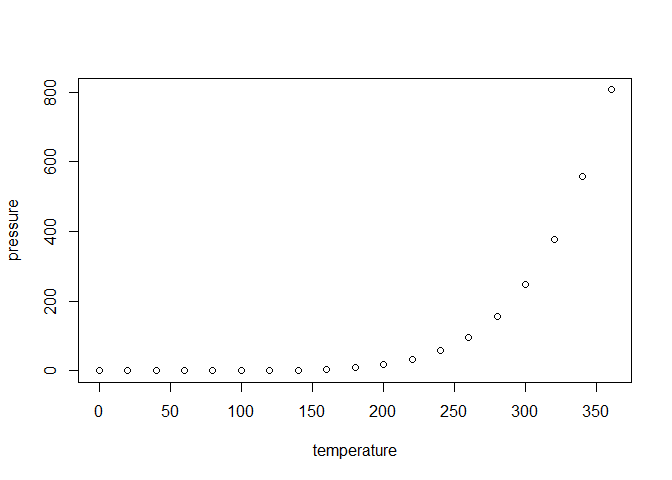
\includegraphics{Class06_files/figure-latex/pressure-1.pdf}

Note that the \texttt{echo\ =\ FALSE} parameter was added to the code
chunk to prevent printing of the R code that generated the plot.

\hypertarget{our-first-function}{%
\subsection{Our first function}\label{our-first-function}}

This is an example function named \texttt{add} with inpu \texttt{x} and
\texttt{y}

\begin{Shaded}
\begin{Highlighting}[]
\NormalTok{add <-}\StringTok{ }\ControlFlowTok{function}\NormalTok{(x, }\DataTypeTok{y=}\DecValTok{1}\NormalTok{) \{}
  \CommentTok{# Sum the input x and y}
\NormalTok{  x }\OperatorTok{+}\StringTok{ }\NormalTok{y}
\NormalTok{\}}
\end{Highlighting}
\end{Shaded}

Lets try using it

\begin{Shaded}
\begin{Highlighting}[]
\KeywordTok{add}\NormalTok{(}\DataTypeTok{x=}\KeywordTok{c}\NormalTok{(}\DecValTok{1}\NormalTok{,}\DecValTok{6}\NormalTok{,}\DecValTok{2}\NormalTok{), }\DataTypeTok{y=}\DecValTok{4}\NormalTok{)}
\end{Highlighting}
\end{Shaded}

\begin{verbatim}
## [1]  5 10  6
\end{verbatim}

A second example function to re-scale data to lie between 0 and 1

\begin{Shaded}
\begin{Highlighting}[]
\NormalTok{rescale <-}\StringTok{ }\ControlFlowTok{function}\NormalTok{(x) \{}
\NormalTok{  rng <-}\StringTok{ }\KeywordTok{range}\NormalTok{(x)}
\NormalTok{  (x }\OperatorTok{-}\StringTok{ }\NormalTok{rng[}\DecValTok{1}\NormalTok{] }\OperatorTok{/}\StringTok{ }\NormalTok{(rng[}\DecValTok{2}\NormalTok{] }\OperatorTok{-}\StringTok{ }\NormalTok{rng[}\DecValTok{1}\NormalTok{]))}
\NormalTok{\}}
\end{Highlighting}
\end{Shaded}

\begin{Shaded}
\begin{Highlighting}[]
\KeywordTok{rescale}\NormalTok{(}\KeywordTok{c}\NormalTok{(}\DecValTok{1}\OperatorTok{:}\DecValTok{10}\NormalTok{, }\OtherTok{NA}\NormalTok{))}
\end{Highlighting}
\end{Shaded}

\begin{verbatim}
##  [1] NA NA NA NA NA NA NA NA NA NA NA
\end{verbatim}

\begin{Shaded}
\begin{Highlighting}[]
\NormalTok{x <-}\StringTok{ }\KeywordTok{c}\NormalTok{(}\DecValTok{1}\OperatorTok{:}\DecValTok{10}\NormalTok{, }\OtherTok{NA}\NormalTok{)}
\NormalTok{rng <-}\StringTok{ }\KeywordTok{range}\NormalTok{(x, }\DataTypeTok{na.rm =} \OtherTok{TRUE}\NormalTok{)}
\NormalTok{rng}
\end{Highlighting}
\end{Shaded}

\begin{verbatim}
## [1]  1 10
\end{verbatim}

Mix for missing values NAs

\begin{Shaded}
\begin{Highlighting}[]
\NormalTok{rescale2 <-}\StringTok{ }\ControlFlowTok{function}\NormalTok{(x) \{}
\NormalTok{  rng <-}\StringTok{ }\KeywordTok{range}\NormalTok{(x, }\DataTypeTok{na.rm =} \OtherTok{TRUE}\NormalTok{)}
\NormalTok{  (x }\OperatorTok{-}\StringTok{ }\NormalTok{rng[}\DecValTok{1}\NormalTok{] }\OperatorTok{/}\StringTok{ }\NormalTok{(rng[}\DecValTok{2}\NormalTok{] }\OperatorTok{-}\StringTok{ }\NormalTok{rng[}\DecValTok{1}\NormalTok{]))}
\NormalTok{\}}
\end{Highlighting}
\end{Shaded}

\begin{Shaded}
\begin{Highlighting}[]
\KeywordTok{rescale2}\NormalTok{(}\KeywordTok{c}\NormalTok{(}\DecValTok{1}\OperatorTok{:}\DecValTok{10}\NormalTok{, }\OtherTok{NA}\NormalTok{))}
\end{Highlighting}
\end{Shaded}

\begin{verbatim}
##  [1] 0.8888889 1.8888889 2.8888889 3.8888889 4.8888889 5.8888889 6.8888889
##  [8] 7.8888889 8.8888889 9.8888889        NA
\end{verbatim}

\begin{Shaded}
\begin{Highlighting}[]
\NormalTok{rescale3 <-}\StringTok{ }\ControlFlowTok{function}\NormalTok{(x, }\DataTypeTok{na.rm=}\OtherTok{TRUE}\NormalTok{, }\DataTypeTok{plot=}\OtherTok{FALSE}\NormalTok{) \{}
 \ControlFlowTok{if}\NormalTok{(na.rm) \{}
\NormalTok{ rng <-}\KeywordTok{range}\NormalTok{(x, }\DataTypeTok{na.rm=}\NormalTok{na.rm)}
\NormalTok{ \} }\ControlFlowTok{else}\NormalTok{ \{}
\NormalTok{ rng <-}\KeywordTok{range}\NormalTok{(x)}
\NormalTok{ \}}
 \KeywordTok{print}\NormalTok{(}\StringTok{"Hello"}\NormalTok{)}
\NormalTok{ answer <-}\StringTok{ }\NormalTok{(x }\OperatorTok{-}\StringTok{ }\NormalTok{rng[}\DecValTok{1}\NormalTok{]) }\OperatorTok{/}\StringTok{ }\NormalTok{(rng[}\DecValTok{2}\NormalTok{] }\OperatorTok{-}\StringTok{ }\NormalTok{rng[}\DecValTok{1}\NormalTok{])}
 \KeywordTok{print}\NormalTok{(}\StringTok{"is it me you are looking for?"}\NormalTok{)}
 \ControlFlowTok{if}\NormalTok{(plot) \{}
   \KeywordTok{print}\NormalTok{(}\StringTok{"Please stop singing!"}\NormalTok{)}
 \KeywordTok{plot}\NormalTok{(answer, }\DataTypeTok{typ=}\StringTok{"b"}\NormalTok{, }\DataTypeTok{lwd=}\DecValTok{4}\NormalTok{)}
\NormalTok{ \}}
 \KeywordTok{print}\NormalTok{(}\StringTok{"I can see it in ..."}\NormalTok{)}
\NormalTok{\}}
\end{Highlighting}
\end{Shaded}

\begin{Shaded}
\begin{Highlighting}[]
\KeywordTok{rescale3}\NormalTok{(x, }\DataTypeTok{plot=}\OtherTok{TRUE}\NormalTok{)}
\end{Highlighting}
\end{Shaded}

\begin{verbatim}
## [1] "Hello"
## [1] "is it me you are looking for?"
## [1] "Please stop singing!"
\end{verbatim}

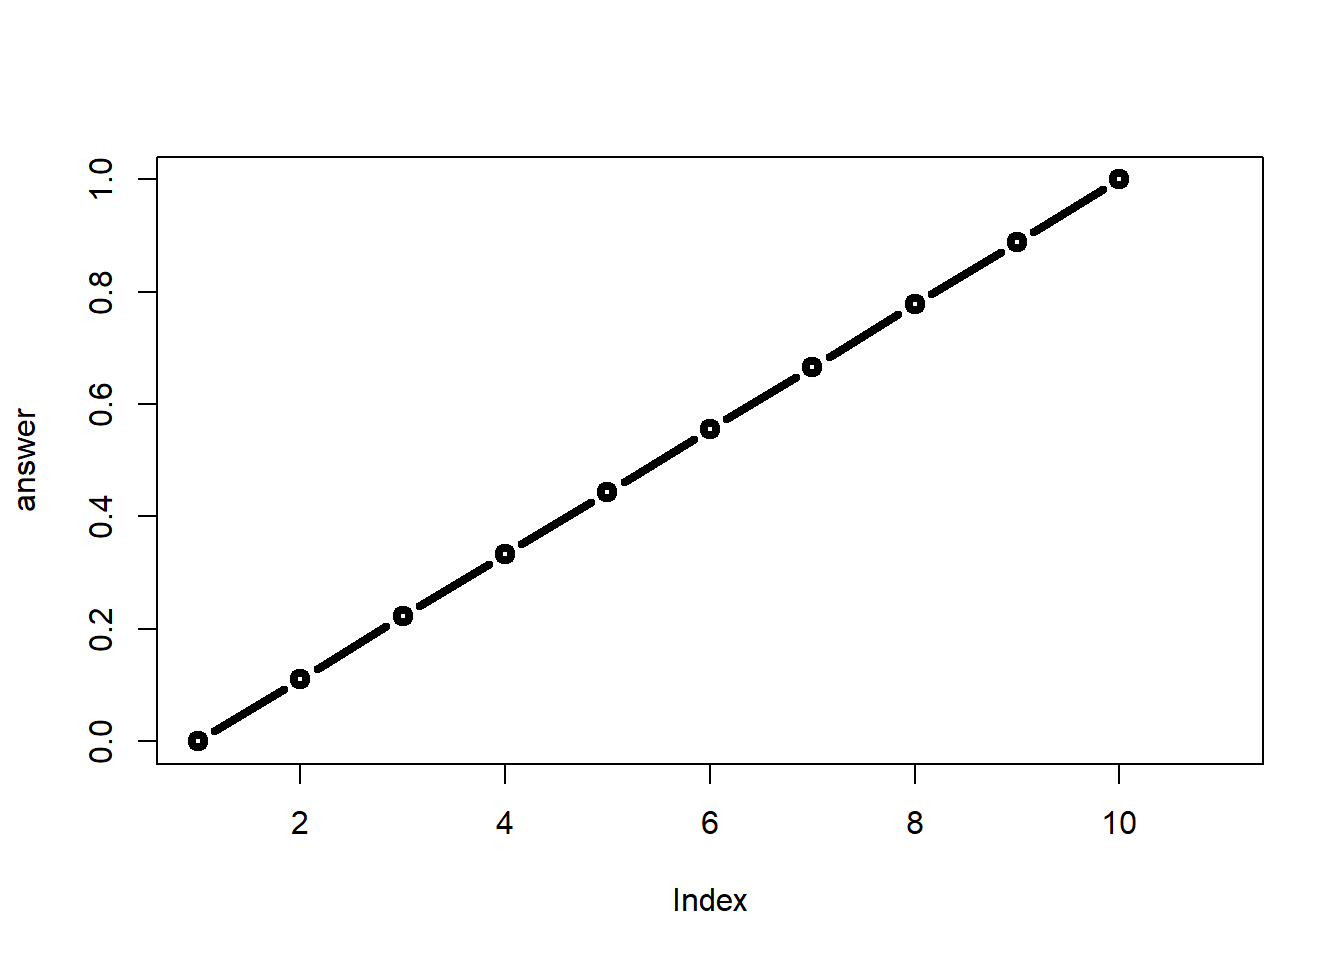
\includegraphics{Class06_files/figure-latex/unnamed-chunk-14-1.pdf}

\begin{verbatim}
## [1] "I can see it in ..."
\end{verbatim}

\end{document}
